\chapter{The Math Toolkit}
This module teaches every piece of math used later in the course. If you already know it, skim the worked examples and move on.

\section{Big and small numbers (scientific notation)}
\begin{kid}
Light is \emph{so} fast that it could go around the Earth about seven times in one second. To write such big numbers --- and tiny ones like ``one billionth of a second'' --- scientists use a shortcut: count the zeros and write that count as a little number up high. $10^3$ means 1 followed by 3 zeros = 1000. $10^{-3}$ means ``1 divided into 1000 pieces'' = 0.001.
\end{kid}

\begin{keyeq}{Scientific notation}
\[ N = m \times 10^{k} \qquad\text{and}\qquad 10^{a}\times10^{b}=10^{a+b} \]
\begin{symbols}
$N$ & the number being written & any\\
$m$ & the \emph{mantissa}, a number between 1 and 10 & ---\\
$k$ & the power of ten (how many places to move the decimal point; negative = move left) & ---\\
$a,b$ & any two exponents; multiplying powers of ten adds the exponents & ---\\
\end{symbols}
\end{keyeq}

\begin{center}\small
\begin{tabular}{llll}\toprule
Prefix & Symbol & Factor & Light travels about\dots\\\midrule
milli & m & $10^{-3}$ & 300 km in 1 ms\\
micro & $\mu$ & $10^{-6}$ & 300 m in 1 $\mu$s\\
nano & n & $10^{-9}$ & 30 cm in 1 ns\\
pico & p & $10^{-12}$ & 0.3 mm in 1 ps\\\bottomrule
\end{tabular}\end{center}

\begin{worked}{multiplying with powers of ten}
\textbf{Given:} speed $c = 2.997\times10^{8}$ m/s, time $t = 4.00\times10^{-7}$ s. Find $c\times t$.
\step{Step 1 --- multiply the mantissas} $2.997\times4.00 = 11.988$
\step{Step 2 --- add the exponents} $10^{8}\times10^{-7}=10^{8+(-7)}=10^{1}$
\step{Step 3 --- combine} $11.988\times10^{1} = 119.88$ m
\result{$c\,t = 119.88$ m.}
\end{worked}

\section{Angles: degrees and radians}
\fig[0.6]{radians}{A radian is the angle whose arc is exactly one radius long.}

\begin{kid}
Imagine a pizza. If you cut a slice whose crust is exactly as long as the line from the center to the crust, that slice's angle is \textbf{one radian}. A whole pizza has a bit more than 6 of those slices (6.28, which is $2\pi$).
\end{kid}

\begin{keyeq}{Degree--radian conversion and arc length}
\[ \theta_{\text{rad}} = \theta_{\text{deg}}\times\frac{\pi}{180} \qquad\qquad s = r\,\theta_{\text{rad}} \]
\begin{symbols}
$\theta_{\text{deg}}$ & an angle in degrees (a full circle = 360°) & degrees\\
$\theta_{\text{rad}}$ & the same angle in radians (a full circle = $2\pi$) & radians\\
$\pi$ & 3.14159\dots, ratio of a circle's circumference to its diameter & ---\\
$r$ & radius (in LiDAR: the range to the target) & m\\
$s$ & arc length: how far you move along the circle & m\\
\end{symbols}
\end{keyeq}

Why care? Because \textbf{sideways error = range $\times$ angle error (in radians)}. This ``small-angle rule'' will appear in nearly every module. It works because for small angles the arc and the straight sideways distance are almost identical ($\sin\theta\approx\tan\theta\approx\theta$ for $\theta$ in radians).

\begin{worked}{a tiny angle at a long range}
\textbf{Given:} an aiming error of 20 arc-seconds at 100 m.
\step{Step 1 --- seconds to degrees} $20'' = 20/3600 = 0.005556^\circ$
\step{Step 2 --- degrees to radians} $0.005556\times\pi/180 = 9.70\times10^{-5}$ rad
\step{Step 3 --- arc length} $s = 100\times9.70\times10^{-5} = 0.0097$ m
\result{about 1 cm sideways --- the classic surveyor's rule ``20 seconds at 100 m is a centimeter.''}
\end{worked}

\section{Sine and cosine}
\fig[0.38]{unitcircle}{On a circle of radius 1, cosine is the ``across'' part and sine is the ``up'' part.}

\begin{kid}
Lean a 1-meter stick against a wall. The bottom of the stick is some distance from the wall (that is \textbf{cosine}) and the top is some height up the wall (that is \textbf{sine}). If the stick leans a lot, cosine is big and sine is small. If it stands almost straight up, sine is big and cosine is small.
\end{kid}

\begin{keyeq}{Right-triangle trigonometry}
\[ \text{across} = L\cos\theta,\qquad \text{up}=L\sin\theta,\qquad L=\sqrt{\text{across}^2+\text{up}^2},\qquad \theta=\operatorname{atan2}(\text{up},\text{across}) \]
\begin{symbols}
$L$ & length of the slanted side (hypotenuse) & m\\
$\theta$ & angle measured from the ``across'' direction & deg or rad\\
$\cos,\sin$ & functions that turn an angle into a number between $-1$ and $+1$ & ---\\
atan2 & ``two-argument arctangent'': returns the angle and gets the quadrant right & rad\\
\end{symbols}
\end{keyeq}

\begin{worked}{a 3-4-5 triangle}
\textbf{Given:} a slope distance of 5.000 m at an angle of 36.87° above horizontal.
\step{Step 1} across $=5.000\cos 36.87^\circ = 5.000\times0.8000 = 4.000$ m
\step{Step 2} up $=5.000\sin 36.87^\circ = 5.000\times0.6000 = 3.000$ m
\step{Step 3 (check)} $\sqrt{4^2+3^2}=\sqrt{25}=5$ \checkmark
\result{4.000 m across and 3.000 m up.}
\end{worked}

\section{Vectors}
\begin{minipage}{0.48\linewidth}
\begin{kid}
A vector is an arrow: it says \emph{how far} and \emph{which way}. ``Walk 3 steps east and 1 step north'' is a vector. Two walks one after the other add up to one bigger walk.
\end{kid}
\end{minipage}\hfill
\begin{minipage}{0.48\linewidth}\centering
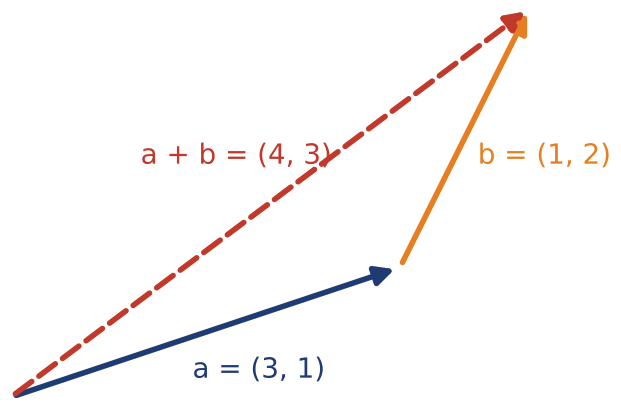
\includegraphics[width=\linewidth]{vectors}
\end{minipage}

\begin{eng}
A 3-D vector is written $\vect{v}=(v_x,v_y,v_z)^\mathsf{T}$. Vectors add component by component. Its length (norm) is $\|\vect{v}\|=\sqrt{v_x^2+v_y^2+v_z^2}$. Two products appear later:
\[ \vect{a}\cdot\vect{b}=a_xb_x+a_yb_y+a_zb_z \quad(\text{dot: a number}),\qquad
\vect{a}\times\vect{b}=\begin{pmatrix}a_yb_z-a_zb_y\\ a_zb_x-a_xb_z\\ a_xb_y-a_yb_x\end{pmatrix}\quad(\text{cross: a vector}). \]
The dot product measures how much two arrows point the same way. The cross product is perpendicular to both, and its length equals the area of the parallelogram they span --- which is why LIO-SAM uses it to measure distances to lines and planes (Module 11).
\end{eng}

\begin{worked}{dot and cross products}
\textbf{Given:} $\vect{a}=(1,2,0)$, $\vect{b}=(3,0,0)$.
\step{Dot} $1\cdot3+2\cdot0+0\cdot0 = 3$
\step{Cross} $(2\cdot0-0\cdot0,\ 0\cdot3-1\cdot0,\ 1\cdot0-2\cdot3)=(0,0,-6)$
\step{Meaning} The parallelogram spanned by $\vect a$ and $\vect b$ has area $\|(0,0,-6)\|=6$; with base $\|\vect b\|=3$ its height is $6/3=2$ --- exactly the distance from the tip of $\vect a$ to the line along $\vect b$.
\result{dot = 3, cross = (0, 0, $-$6), point-to-line distance = 2.}
\end{worked}

\section{Matrices in one page}
\begin{eng}
A matrix is a table of numbers that transforms a vector. Multiplying a $3\times3$ matrix by a vector gives a new vector whose each entry is a row of the matrix ``dotted'' with the vector:
\[\begin{pmatrix}a&b&c\\d&e&f\\g&h&i\end{pmatrix}\begin{pmatrix}x\\y\\z\end{pmatrix}=\begin{pmatrix}ax+by+cz\\dx+ey+fz\\gx+hy+iz\end{pmatrix}.\]
Key facts used later: the \textbf{transpose} $\vect{A}^\mathsf{T}$ swaps rows and columns; the \textbf{identity} $\vect I$ changes nothing; the \textbf{inverse} $\vect A^{-1}$ undoes $\vect A$; for a \emph{rotation} matrix the inverse is simply the transpose, $\vect R^{-1}=\vect R^\mathsf{T}$.
\end{eng}

\begin{worked}{matrix times vector}
$\begin{pmatrix}2&0&1\\0&1&0\\1&0&3\end{pmatrix}\begin{pmatrix}1\\4\\2\end{pmatrix}
=\begin{pmatrix}2\cdot1+0\cdot4+1\cdot2\\0\cdot1+1\cdot4+0\cdot2\\1\cdot1+0\cdot4+3\cdot2\end{pmatrix}=\begin{pmatrix}4\\4\\7\end{pmatrix}$
\end{worked}

\section{Statistics: mean, standard deviation, RMSE}
\fig[0.75]{gaussian}{Random measurement errors usually follow a bell curve. About 68\% fall within one standard deviation $\sigma$ and 95\% within 1.96$\sigma$.}

\begin{kid}
Throw ten paper balls at a target. The \textbf{mean} tells you where they landed on average (are you aiming too far left?). The \textbf{spread} (standard deviation) tells you how scattered they are. A great thrower has a mean right on the bullseye \emph{and} a small spread.
\end{kid}

\begin{keyeq}{Mean, standard deviation, RMSE}
\[ \bar e=\frac1n\sum_{i=1}^{n}e_i,\qquad
s=\sqrt{\frac{1}{n-1}\sum_{i=1}^{n}(e_i-\bar e)^2},\qquad
\text{RMSE}=\sqrt{\frac1n\sum_{i=1}^{n}e_i^2} \]
\begin{symbols}
$e_i$ & the $i$-th error (measured minus true) & m\\
$n$ & how many errors we have & ---\\
$\sum$ & ``add them all up,'' from $i=1$ to $n$ & ---\\
$\bar e$ & mean error = \emph{bias} (systematic part) & m\\
$s$ & sample standard deviation = \emph{precision} (random part); $n-1$ because one degree of freedom was spent computing $\bar e$ & m\\
RMSE & root-mean-square error = total \emph{accuracy}; combines bias and spread: $\text{RMSE}^2\approx\bar e^2+s^2$ & m\\
\end{symbols}
\end{keyeq}

\begin{worked}{five elevation errors}
\textbf{Given:} errors $+2, -1, +3, 0, +1$ cm.
\step{Mean} $(2-1+3+0+1)/5 = 5/5 = 1.0$ cm (a 1 cm high bias)
\step{Deviations from mean} $1,-2,2,-1,0$; squares $1,4,4,1,0$; sum $=10$
\step{Std.\ dev.} $s=\sqrt{10/4}=\sqrt{2.5}=1.58$ cm
\step{RMSE} squares of errors $4,1,9,0,1$; sum $=15$; RMSE $=\sqrt{15/5}=\sqrt3=1.73$ cm
\step{Check} $\bar e^2+s^2\cdot\tfrac{n-1}{n}=1+2.5\times0.8=3.0=\text{RMSE}^2$ \checkmark
\result{bias 1.0 cm, precision 1.58 cm, accuracy (RMSE) 1.73 cm.}
\end{worked}

\section{Adding independent errors: root-sum-square}
\begin{keyeq}{Propagation of independent errors}
\[ \sigma_{\text{total}}=\sqrt{\sigma_1^2+\sigma_2^2+\cdots+\sigma_k^2} \]
\begin{symbols}
$\sigma_j$ & standard deviation of the $j$-th independent error source & m\\
$\sigma_{\text{total}}$ & standard deviation of their sum & m\\
\end{symbols}
\end{keyeq}
Errors do \emph{not} add like ordinary numbers because random errors partly cancel. Two independent 3 cm and 4 cm errors combine to $\sqrt{9+16}=5$ cm, not 7 cm. The rule only holds when the sources are \emph{independent}; a systematic error that pushes every point the same way must be treated separately (see Module 13).

\begin{tryit}
\textbf{2.1} Convert 0.05° to radians, then find the sideways error it causes at 80 m.\\
\textbf{2.2} Compute $\sqrt{2^2+1.5^2+3^2}$.\\
\textbf{2.3} A wall is 12 m across and 5 m up from you along the slope. How long is the slope distance?\\
\textbf{2.4} (Simple) You need 3 big steps forward and then 4 big steps to the right. If you could walk straight there instead, how many steps would it be?
\end{tryit}

\sources{Ghilani, C.\ D.\ (2017), \emph{Adjustment Computations: Spatial Data Analysis}, 6th ed., Wiley (statistics, RMSE, propagation); NIST SP 811, \emph{Guide for the Use of the International System of Units}.}
